\section{Input Reduction}
\label{sec:method}

To explain model predictions using a set of important words, we must first
define importance. After defining input perturbation and gradient-based
approximation, we describe input reduction with these importance
metrics. Input reduction 
drastically shortens inputs without causing the model to change its
prediction or significantly decrease its confidence.
Crowdsourced experiments confirm that
reduced examples appear nonsensical to humans: input reduction uncovers
pathological model behaviors.

\subsection{Importance from Input Gradient} 

\citet{ribeiro2016lime} and \citet{li2016understanding} define importance by
seeing how confidence changes when a feature is removed: if removing a feature drastically changes a prediction, it must have been important.  A natural
approximation is to use the gradient~\cite{baehrens2010explain,
simonyan2013deep}.  We formally define these importance metrics in natural
language contexts and introduce the efficient gradient-based approximation.
For each word
in an input sentence, we measure its importance by the change in the
confidence of the original prediction when we remove that word from the sentence.
We switch the sign so that when the confidence decreases, the importance
value is positive.

Formally,
let $\mb{x}=\langle x_1, x_2, \ldots x_n \rangle$ denote the input sentence,
$f(y \g \mb{x})$ the predicted probability of label $y$, and 
$y=\argmax_{y'} f(y' \g \mb{x})$ the original predicted label. The importance is
then
\begin{equation} \label{eq:importance}
    g(x_i\mid \mb{x}) = f(y \g \mb{x}) - f(y \g \mb{x}_{-i}).
\end{equation}
To calculate the importance of each word in a sentence with $n$ words,
we need $n$ forward passes of the model, each time with
one of the words left out.  This is highly inefficient, especially for
longer sentences. Instead, we approximate the importance value with the input
gradient. For each word in the sentence, we calculate the dot product of its
word embedding and the gradient of the output with respect to continuous vector that represents the word: the embedding. The
importance of $n$ words can thus be computed with a single forward-backward
pass. This gradient approximation has been used for various interpretation
methods for natural language classification models~\cite{li2016visualizing,
arras2016explaining}; see \citet{ebrahimi2017hotflip} for further details on the
derivation. We use this approximation in all our experiments as it selects the
same words for removal as an exhaustive search (no approximation). 



\subsection{Removing Unimportant Words}

Instead of looking at the words with high importance values---what
interpretation methods commonly do---we take a complementary approach and study
how the model behaves when the supposedly unimportant words are removed.  
Intuitively, the important words should remain after the unimportant ones are
removed.

Our input reduction process iteratively removes the unimportant words. At each step,
we remove the word with the lowest importance value until the model changes its
prediction.
We experiment with three popular datasets:
\squad~\cite{rajpurkar2016squad} for reading comprehension,
\snli~\cite{bowman2015snli} for textual entailment,
and \vqa~\cite{antol2015vqa} for visual question answering. We describe each of
these tasks and the model we use below, providing full details in the
Supplement.

In \squad, each example is a context paragraph and a question. The task is to
predict a span in the paragraph as the answer.  We reduce only the question
while keeping the context paragraph unchanged. The model we use is the
\abr{DrQA} Document Reader~\cite{chen2017drqa}.

In \snli, each example consists of two sentences: a premise and a hypothesis.
The task is to predict one of three relationships: entailment, neutral, or
contradiction. We reduce only the hypothesis while keeping the premise
unchanged.  The model we use is Bilateral Multi-Perspective
Matching (\abr{BiMPM})~\cite{wang2017bilateral}.

In \vqa, each example consists of an image and a natural language question.
We reduce only the question while keeping the image unchanged. The model we use
is Show, Ask, Attend, and Answer~\cite{kazemi2017show}.

During the iterative reduction process, we ensure that the prediction does not
change (exact span for \squad{}); consequently, the model accuracy
on the reduced examples is identical to the original. The predicted label is
used for input reduction and the ground-truth is never revealed. We use the
validation set for all three tasks.

\begin{figure}[t]
\small

\tikz\node[fill=white!90!colorsnli,inner sep=1pt,rounded corners=0.3cm]{
\begin{tabular}{lp{0.7\columnwidth}}
\textbf{\snli} & \\
Premise & Well dressed man and woman dancing in the street \\
Original & Two man is dancing on the street \\
Reduced & dancing \\
Answer & Contradiction \\
Confidence & 0.977 $\to$ 0.706 \\
\end{tabular}
}; 

\tikz\node[fill=white!90!colorvqa,inner sep=1pt,rounded corners=0.3cm]{
\begin{tabular}{lp{0.7\columnwidth}}
\textbf{\vqa} & \\
& 
\includegraphics[height=1in]{vqa_example} \\
Original & What color is the flower ? \\
Reduced & flower ? \\
Answer & yellow \\
Confidence & 0.827 $\to$ 0.819  \\
\end{tabular}
}; 
\caption{Examples of original and reduced inputs where the models predict the
    same \emph{Answer}. \emph{Reduced} shows the input after reduction.  We
    remove words from the hypothesis for \snli{}, questions for \squad{} and
    \vqa{}.  Given the nonsensical reduced inputs, humans would not be able to
    provide the answer with high confidence, yet, the neural models do.}
\label{fig:reduced_examples}
\end{figure}

Most reduced inputs are nonsensical to humans
(Figure~\ref{fig:reduced_examples}) as they lack information for \emph{any}
reasonable human prediction. However, models make confident predictions, at
times even more confident than the original.

To find the shortest possible reduced inputs (potentially the most meaningless),
we relax the requirement of removing only the least important word and
augment input reduction with beam search. We limit the removal to
the $k$\ \ least important words, where $k$ is the beam size, and decrease the beam
size as the remaining input is shortened.\footnote{We set beam size to $\max(1,
\min(k, L - 3))$ where $k$ is maximum beam size and $L$ is the current length of
the input sentence.} We empirically select beam size five as it produces
comparable results to larger beam sizes with reasonable computation cost. The
requirement of maintaining model prediction is unchanged.
  
\begin{figure*}[t]
    \centering
    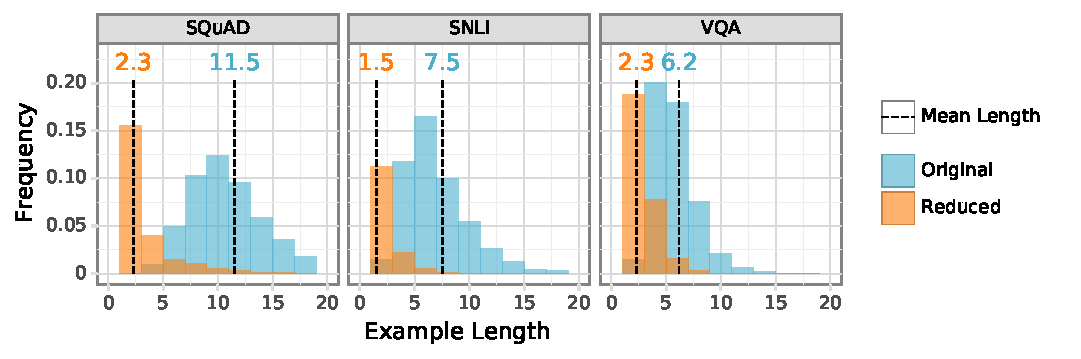
\includegraphics[width=.8\textwidth]{length_histogram}
    \caption{Distribution of input sentence length before and after reduction.
    For all three tasks, the input is often reduced to one or two words without
    changing the model's prediction.}
    \label{fig:lengths_histogram}
\end{figure*}

\begin{figure}[t]
    \centering
    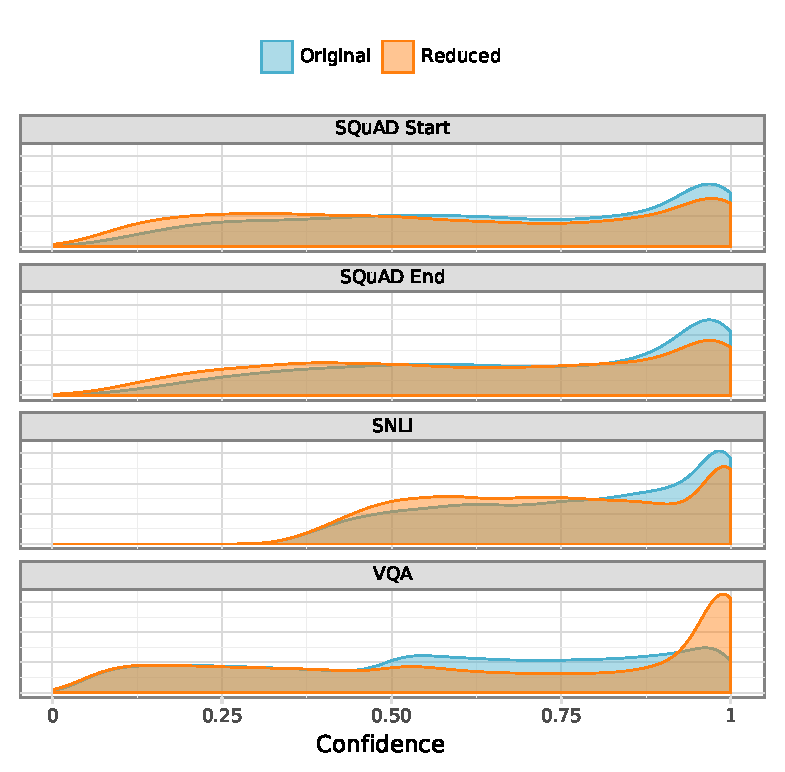
\includegraphics[width=0.5\textwidth]{confidence}
\caption{Density distribution of model confidence on reduced inputs
    is similar to the original confidence.  In \squad, we predict
    the beginning and the end of the answer span, so we show the
    confidence for both.}
    \label{fig:confidence_density}
\end{figure}

With beam search, input reduction finds extremely short reduced examples with
little to no decrease in the model's confidence on its original
predictions.  Figure~\ref{fig:lengths_histogram} compares the length of input
sentences before and after the reduction. For all three tasks, we can often
reduce the sentence to only one word. Figure~\ref{fig:confidence_density}
compares the model's confidence on original and reduced inputs.  On \squad{} and
\snli{} the confidence decreases slightly, and on \vqa{} the confidence even
increases.

\begin{table}[t]
\centering
\begin{tabular}{lccc}
Dataset & Original & Reduced & vs.\ Random \\
\midrule
\squad  & 80.58 & 31.72 & 53.70 \\
\snli-E & 76.40 & 27.66 & 42.31 \\
\snli-N & 55.40 & 52.66 & 50.64 \\
\snli-C & 76.20 & 60.60 & 49.87 \\
\vqa    & 76.11 & 40.60 & 61.60 \\
\end{tabular}
\caption{Human accuracy on \emph{Reduced} examples drops
    significantly compared to the \emph{Original} examples, however, model
    predictions are identical. The reduced examples also appear random to
    humans---they do not prefer them over random inputs
    (\emph{vs.\ Random}).  For \squad, accuracy is reported using F1
    scores, other numbers are percentages. For
    \snli, we report results on the three classes separately: entailment
    (\emph{-E}), neutral (\emph{-N}), and contradiction (\emph{-C}).}
\label{table:human_results}
\end{table}

\subsection{Humans Confused by Reduced Inputs}
\label{sec:human}

On the reduced examples, the models retain their original predictions
despite short input lengths. The following experiments examine whether
these predictions are justified or pathological, based on how humans react to
the reduced inputs.

For each task, we sample 200 examples that are correctly classified by
the model and generate their reduced examples. In the first setting, we
compare the human accuracy on original and reduced examples.
We recruit two groups of crowd workers and task them with textual entailment,
reading comprehension, or visual question answering. We show one group the
original inputs and the other the reduced.  Humans are no longer able to give
the correct answer, showing a significant accuracy loss on all three tasks
(compare \emph{Original} and \emph{Reduced} in Table~\ref{table:human_results}).

The second setting examines how random the reduced examples appear to
humans. For each of the original examples, we generate a version where words are
randomly removed until the
length matches the one generated by input reduction. We present the original example
along with the two reduced examples and ask crowd workers their preference between the two
reduced ones. The workers' choice is almost fifty-fifty (the \emph{vs.\ Random}
in Table~\ref{table:human_results}): the reduced examples appear almost
random to humans.

These results leave us with two puzzles: why are the models highly confident on the
nonsensical reduced examples? And why, when the \loo{} method selects important
words that appear reasonable to humans, the input reduction process selects ones
that are nonsensical?
